% This is part of Un soupçon de mathématique sans être agressif pour autant
% Copyright (c) 2012
%   Laurent Claessens
% See the file fdl-1.3.txt for copying conditions.

\begin{exercice}\label{exoSeconde-0035}

Dans l'histogramme suivant, l'effectif de la classe $[17;19[$ est égal à 2.

\begin{center}
  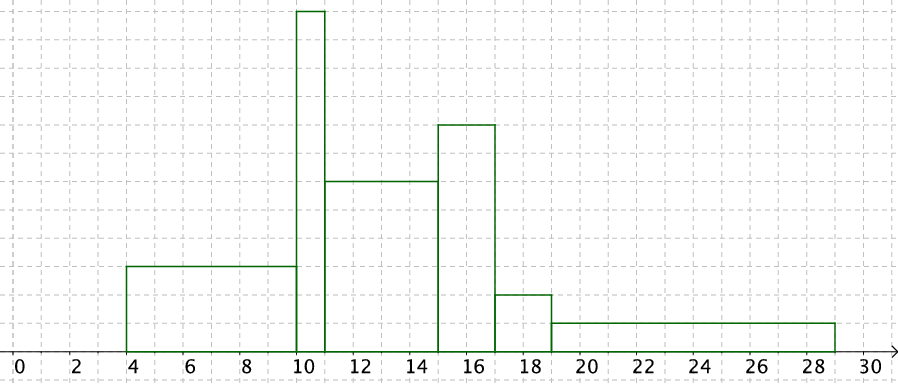
\includegraphics[width=10cm]{DS8_Fig_Ex1}
\end{center}

\begin{enumerate}
\item Faire un tableau décrivant les effectifs de chaque classe. 
\item Quelle est la classe modale de cette série ?
\end{enumerate}


\corrref{Seconde-0035}
\end{exercice}
